\section{Pendahuluan}
\subsection{Latar Belakang}
Pada Wireless Jaringan Komputer, terdapat setidaknya 3 jenis, yaitu Point-to-Point Protocol
(PPP), Point-to-multipoint dan Wireless Bridging.\\\\
Point-to-Point Protocol (PPP) adalah data link protokol yang umum digunakan dalam
membangun hubungan langsung antara dua node jaringan. Hal ini dapat menyediakan koneksi
otentikasi, transmisi enkripsi (menggunakan ECP, RFC 1968), dan kompresi. Jenis ini
biasanya digunakan untuk menghubungkan jaringan antar 2 gedung atau antar 2 BTS (Base
Transceiver Station).\\\\
Point-to-multipoint adalah pendekatan yang paling populer untuk komunikasi nirkabel yang
memiliki banyak node, tujuan akhir atau pengguna akhir. Jenis ini biasanya digunakan untuk
membuat wifi atau hotspot yang berasal dari 1 sumber disebar ke banyak client dalam suatu
jaringan.\\\\
Wireless Bridging digunakan untuk menghubungkan dua segmen LAN melalui tautan
nirkabel. Kedua segmen akan berada di subnet yang sama dan terlihat seperti dua switch
Ethernet yang dihubungkan oleh kabel ke semua komputer di subnet.\\\\
Untuk mengembangkan jaringan komputer berbasis wireless yang berkualitas dan mempunyai
ketersediaan tinggi, penggunaan 3 jenis ini perlu disesuaikan dengan kebutuhan dan kondisi
nya, sehingga kali ini saya akan membahasnya 1 persatu dari 3 jenis koneksi wireless
tersebut.

%\begin{itemize}[label=$\bullet$, itemsep=-1pt, leftmargin=*]
%	\item Cek Halo
%\end{itemize}

\subsection{Maksud dan Tujuan}
Mengetahui dan memahami 3 jenis koneksi pada Jaringan Wireless.

\subsection{Hasil yang diharapkan}
Dapat mengkonfigurasi koneksi Wireless Bridge, Point to Point dan Point to Multipoint
dengan tepat.

%===========================================================%
\section{Tugas Pendahuluan}
\begin{enumerate}
	\item Halo
\end{enumerate}

\begin{center}
	\colorbox{cyan!30}{\parbox{0.8\linewidth}{\textbf{Opsional:} Pelajari Git dan Github. Anda dapat memulai pembelajaran dari sumber berikut ini: \\ \href{https://github.com}{GitHub - https://github.com} \\ \href{https://git-scm.com/doc}{Git -https://git-scm.com/doc}}}
\end{center}

%===========================================================%
\section{Alat dan Bahan}
\begin{itemize}[label=$\bullet$, itemsep=-1pt, leftmargin=*]
	\item 2 atau lebih perangkat router mikrotik yang sudah support wireless.
	\item Aplikasi Winbox.
\end{itemize}

%===========================================================%
\section{Jangka Waktu Pelaksanaan}
Pemahaman dan konfigurasi 1 jam.

%===========================================================%
\section{Proses dan Tahapan Konfigurasi}

\subsection{Wireless Point to Point}
Untuk koneksi Point to Point seperti contohnya topologi seperti dibawah ini, biasanya
digunakan untuk menghubungkan 2 router atau 2 node jaringan, Hal ini dilakukan biasanya
untuk koneksi koneksi jarak jauh yang mengharapkan kecepatan tinggi misal untuk
menghubungkan jaringan antar gedung, menghubungkan BTS (Base Transceiver Station) to
BTS (Base Transceiver Station). Koneksi point to point ini akan lebih aman karena maksimal
node yang terhubung hanya 2. Untuk konfigurasinya seperti berikut ini.

\begin{center}
	\begin{enumerate}
		\item Buatlah skenario topologi seperti gambar dibawah ini, Router1 (Router Utama) menjadi mode Bridge dan Router 2 menjadi mode Station.
		\begin{figure}[H]
			\centering
			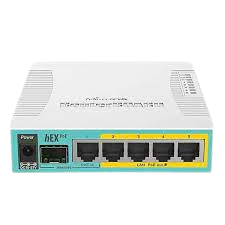
\includegraphics[width=0.7\linewidth]{P1/img/contoh.png}
			\caption{Gambar Contoh}
			\label{fig:gambarcontoh}
		\end{figure}
		\item Konfigurasi wireless mode Bridge pada Router1 seperti berikut ini.
		\begin{figure}[H]
			\centering
			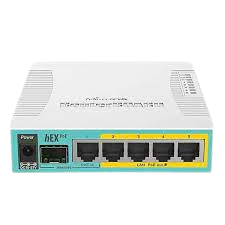
\includegraphics[width=0.7\linewidth]{P1/img/contoh.png}
			\caption{Gambar Contoh}
			\label{fig:gambarcontoh}
		\end{figure}
		\item Untuk konfigurasi IP sesuaikan dengan kebutuhan kalian, saya contohkan seperti dibawah ini.
		\begin{figure}[H]
			\centering
			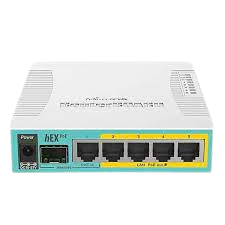
\includegraphics[width=0.7\linewidth]{P1/img/contoh.png}
			\caption{Gambar Contoh}
			\label{fig:gambarcontoh}
		\end{figure}
		\item Pada Router2 konfigurasi mode Station seperti dibawah ini, namun sebelumnya silahkan Scan dan connectkan dengan SSID yang telah diatur di Router1 yaitu PointToPointLur.
		\begin{figure}[H]
			\centering
			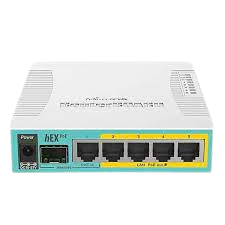
\includegraphics[width=0.7\linewidth]{P1/img/contoh.png}
			\caption{Gambar Contoh}
			\label{fig:gambarcontoh}
		\end{figure}
		\item Setelah itu setting IP yang satu subnet dengan Router1.
		\begin{figure}[H]
			\centering
			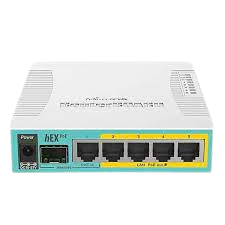
\includegraphics[width=0.7\linewidth]{P1/img/contoh.png}
			\caption{Gambar Contoh}
			\label{fig:gambarcontoh}
		\end{figure}
		\item Selanjutnya silahkan ping IP Router2 dari Router1 seperti berikut ini.
		\begin{figure}[H]
			\centering
			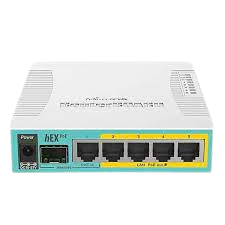
\includegraphics[width=0.7\linewidth]{P1/img/contoh.png}
			\caption{Gambar Contoh}
			\label{fig:gambarcontoh}
		\end{figure}
		\item Ping IP Router1 dari Router2 seperti berikut ini. Jika TTL maka konfigurasi PointToPoint berhasil.
		\begin{figure}[H]
			\centering
			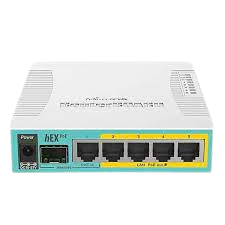
\includegraphics[width=0.7\linewidth]{P1/img/contoh.png}
			\caption{Gambar Contoh}
			\label{fig:gambarcontoh}
		\end{figure}
		\item Tambahan saja, pada Router2 kalian dapat cek di registration Tx dan Rx yang didapat serta kekuatan sinyal seperti berikut.
		\begin{figure}[H]
			\centering
			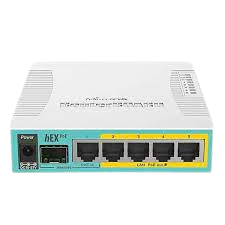
\includegraphics[width=0.7\linewidth]{P1/img/contoh.png}
			\caption{Gambar Contoh}
			\label{fig:gambarcontoh}
		\end{figure}
	\end{enumerate}
\end{center}

\subsection{Wireless Point to Multipoint}
Koneksi ini yang paling banyak digunakan, karena kelebihannya yaitu dapat mengkoneksikan
multipoint atau banyak node dari satu point atau node sumber, penerapan pada koneksi ini
biasanya berupa hotspot. Untuk konfigurasinya seperti berikut.
Untuk gambar topologi sama dengan PointToPoint, hanya saja berbeda di konfigurasi dan
mode pada routernya.
\begin{center}
	\begin{enumerate}
		\item Buatlah mode AP Bridge di router yang dijadikan router utama seperti berikut.
		\item Kemudian setting IP pada wlan1 sesuai keinginan kalian, disini saya konfigurasi IP seperti berikut.
		\item Pada Router Station, pergi ke pengaturan wireless dan lakukan scan, kemudian connectkan dengan SSID yang telah di setting di Router utama yaitu PointToMultiPointLur.
		\item Settingannya seperti berikut.
		\item Lakukan juga konfigurasi IP pada wlan1 yang satu subnet dengan Router Utama.
		\item Setelah itu silahkan cek PING dari router AP Bridge ke station.
		\item PING dari router station ke AP Bridge. Jika TTL maka koneksi telah berhasil terhubung.
		\item Kalian juga bisa menghubungkan laptop kalian ke router1 atau router utama melalui koneksi wifi yang sudah dibuat, pastikan laptop kalian IP nya sudah di setting 1 network, dan lakukan PING dari laptop kalian ke IP Router1 atau router wifi.
	\end{enumerate}
\end{center}

\subsection{Wireless Bridge}
Untuk wireless bridge ini sangatlah sederhana, koneksi ini sangat jarang ditemui pada
implementasi realnya, konfigurasi ini menjadikan seolah-olah koneksi yang terhubung
menggunakan switch, keunggulan yang saya rasakan yaitu ringannya kinerja router yang
menggunakan koneksi ini. Untuk konfigurasinya seperti berikut.
Untuk gambar topologi sama dengan Point To Point, hanya saja berbeda di konfigurasi dan
mode pada routernya.
\begin{center}
	\begin{enumerate}
		\item Setting pada Router1 sebagai mode bridge dan SSID sebagai berikut.
		\item Konfigurasi IP pada interface wlan1 yang terhubung ke router dan ether2 yang terhubung ke Laptop seperti berikut.
		\item Tambahkan bridge pada router1 seperti berikut.
		\item Dan tambahkan Port pada bridge untuk wlan dan ether2, kemudia apply>ok.
		\item Pada Router2, lakukan konfigurasi dengan mode station pseoubridge seperti berikut, setelah itu scan dan konekan dengan SSID yang telah di setting di Router1.
		\item Setting IP pada interface wlan1 yang terhubung ke router dan ether2 yang terhubung ke laptop seperti berikut.
		\item Tambahan saja, untuk anda dapat gunakan access list untuk mengkontrol setiap perangkat yang terhubung dengan MAC.
		\item Lakukan konfigurasi IP pada laptop yg terhubung ke Router1 seperti berikut.
		\item Lakukan konfigurasi IP pada laptop yg terhubung ke Router2 seperti berikut.
		\item Setelah semua terkonfigurasi. Lakukan PING dari kedua router seperti berikut, jika saling TTL maka kedua router telah terhubung.
		\item Lakukan juga PING antar laptop seperti berikut. jika reply maka konfigurasi Wireless Bridge berhasil.
	\end{enumerate}
\end{center}

%===========================================================%
\section{Hasil yang didapat}
Memahami dan mengkonfigurasi koneksi Point to Point, Point to Multipoint dan Wireless
Bridging dengan tepat.

%===========================================================%
\section{Temuan Permasalahan}
Firewall hidup pada Laptop dapat mempengaruhi koneksi wireless tidak terhubung, kalian
bisa menonaktifkan firewall di laptop kalian, tetapi hal ini tidak terjadi di semua perangkat.

%===========================================================%
\section{Kesimpulan}
Dengan memahami dan mengkonfigurasi 3 jenis koneksi pada wireless, kita dapat
mengimplementasikan koneksi wireless dengan tepat sesuai kebutuhan dan kondisi tertentu.

\cite{Newton1687}.